\documentclass[12pt,a4paper]{article}
\usepackage[utf8]{inputenc}
\usepackage[spanish]{babel}
\usepackage{amsmath}
\usepackage{amsfonts}
\usepackage{amssymb}
\usepackage{geometry}
\usepackage{listings}
\usepackage{xcolor}
\usepackage{graphicx}
\usepackage{float}
\usepackage{booktabs}
\geometry{margin=2.5cm}

% Configuración de listings para código R
\lstset{
    basicstyle=\ttfamily\small,
    breaklines=true,
    breakatwhitespace=true,
    frame=single,
    language=R,
    showstringspaces=false,
    columns=flexible
}

\title{Estadística y Diseño de Experimentos\\
Ejercicios 5}
\date{21 de Noviembre, 2025}
\author{}

\begin{document}

\maketitle

\noindent\textbf{Nombre del alumnx:} \underline{\hspace{0.5cm}Martínez Buenrostro Jorge Rafael\hspace{0.5cm}}

\vspace{1cm}

Se estudian tres marcas de insecticidas, sospechando que su porcentaje de efectividad es distinta. Se prueban seis realizaciones de cada marca, obteniendo los siguientes resultados:

% Please add the following required packages to your document preamble:
% \usepackage{booktabs}
\begin{table}[H]
  \centering
  \begin{tabular}{@{}l|llllll@{}}
    \toprule
    Marca 1 & 86.92 & 85.96 & 86.47 & 85.71 & 86.26 & 86.79 \\
    Marca 2 & 83.53 & 84.36 & 82.63 & 82.94 & 83.88 & 83.21 \\
    Marca 3 & 83.88 & 86.18 & 84.87 & 85.70 & 85.21 & 85.66 \\ \bottomrule
  \end{tabular}
  \caption{Cuadro 1: Porcentaje de efectividad}
\end{table}

\begin{enumerate}
  \item Grafique los diagramas de caja y escriba sus primeras impresiones.
  \begin{figure}[H]
    \centering
    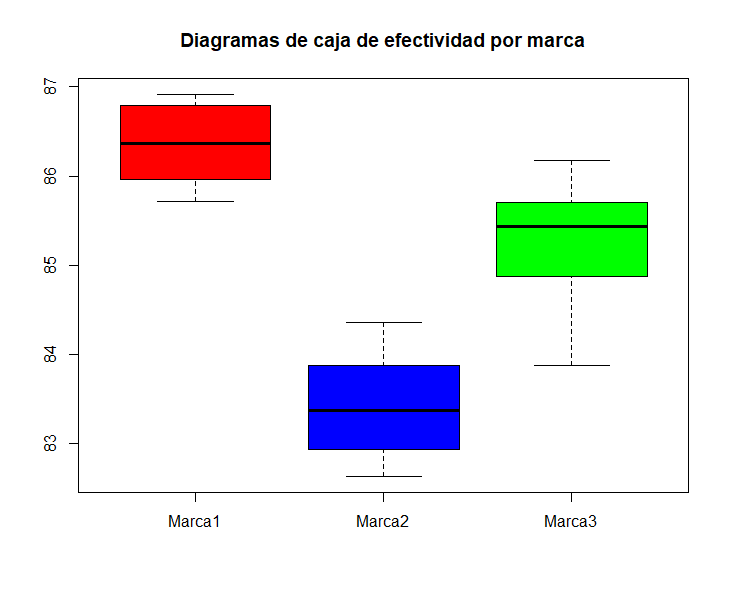
\includegraphics[width=0.6\textwidth]{img/boxplot.png}
  \end{figure}
  
  De los diagramas de caja se observa que la Marca 1 tiene la media de efectividad más alta y la menor variabilidad. La Marca 2 tiene la mayor cantidad de valores con menor efectividad. Mientras que La Marca 3 tiene mayor variabilidad entre sus realizaciones. 

  \item Calcule las medidas importantes:
  \begin{itemize}
    \item Número de tratamientos, m: 3
    \item Número de datos en cada tratamiento i: 6, 6, 6
    \item Número total de datos, N: 18
    \item Valores de cada media muestral \( \overline{X}_i  \): m1=86.35167, m2=83.425, m3=85.25
  \end{itemize}
  \begin{lstlisting}[caption={Código para obtener todas las medidas importantes}]
    m <- 3
    n1 <- length(Marca1); n2 <- length(Marca2); n3 <- length(Marca3)
    N <- n1 + n2 + n3

    m1 <- mean(Marca1); m2 <- mean(Marca2); m3 <- mean(Marca3)
    v1 <- var(Marca1); v2 <- var(Marca2); v3 <- var(Marca3)
  \end{lstlisting}

  \item \textbf{ANOVA} Complete con ayuda de \textbf{R} la siguiente tabla del ANOVA.
  % Please add the following required packages to your document preamble:
  % \usepackage{booktabs}
  \begin{table}[H]
      \centering
      \begin{tabular}{@{}lllll@{}}
      \toprule
      Variabilidad & Suma de Cuadrados & Cuadrados Medios & Estadístico $F_0$ & p-valor \\ \midrule
      Tratamientos & $SC_{TRAT}=26.219$ & $CM_{TRAT}=13.110$ & $F_0=30.89$ & 4.8e-06\\
      ERROR & $SC_{ERROR}=6.367$ & $CM_{ERROR}=0.424$ & & \\ \bottomrule
      \end{tabular}
  \end{table}

  Para poder completar la tabla, se utiliza el siguiente código en R:
  \begin{lstlisting}[caption={Código para completar la tabla ANOVA}]
    Tratamientos<-c(rep("Marca1",6),rep("Marca2",6),rep("Marca3",6))
    Insecticidas<-c(Marca1,Marca2,Marca3)

    Datos<-data.frame(TRATAMIENTOS=Tratamientos,INSECTICIDA=Insecticidas)
    Anova1<-aov(Datos$INS~Datos$TRAT)

    summary(Anova1)
  \end{lstlisting}

  \item Usando un nivel de significancia \(\alpha=0.05\), decida si se rechaza o no la hipótesis nula en el ANOVA. \textbf{Dé una interpretación}. 
  
  Primero tomamos el valor de \(F_0\) de la tabla ANOVA, \( F_0 =  30.89 \). Se rechaza \( H_0 \) si \( F_0 > F_{\alpha,(m-1),(N-m)} \). El valor del cuantil lo podemos obtener en R con el siguiente código: \texttt{qf(1 - alpha, m-1, N-m)}, lo que nos da la siguiente desigualdad \( 30.89 > 3.68232 \). Por lo tanto, se rechaza la hipótesis nula \( H_0 \). Esto significa que existen diferencias significativas entre al menos dos de las marcas de insecticidas e cuanto a su efectividad.

  \item Si se rechaza la hipótesis nula en el inciso anterior, haga las múltiples comparaciones para las medias mediante el método LSD. Utilice para este punto, \(\alpha=0.05\). \textbf{Dé una interpretación}
  
  Para hacer las comparaciones múltiples, se utiliza el siguiente código en R:
  \begin{lstlisting}
    l12 <- abs(m1 - m2) / sqrt(CME * (1/n1 + 1/n2))
    l13 <- abs(m1 - m3) / sqrt(CME * (1/n1 + 1/n3))
    l23 <- abs(m2 - m3) / sqrt(CME * (1/n2 + 1/n3))
  \end{lstlisting}
  Estas comparaciones nos da el valor de \it{l} para cada una de las comparaciones. Ahora se necesita el valor del cuantil \( t_{\frac{\alpha}{2},N-m} \). Recorndando que se rechaza \(H_0\) si \(|l| > t_{\frac{\alpha}{2},N-m}\).

  Las comparaciones son las siguientes:
  % Please add the following required packages to your document preamble:
  % \usepackage{booktabs}
  \begin{table}[H]
    \centering
    \begin{tabular}{@{}cc@{}}
    \toprule
    Comparación de medias & Valores ($l > t$)            \\ \midrule
    $\mu_1$ vs $\mu_2$    & 2.1314 \textgreater 7.780684 \\
    $\mu_1$ vs $\mu_3$    & 2.1314 \textgreater 2.928834 \\
    $\mu_2$ vs $\mu_3$    & 2.1314 \textgreater 4.85185  \\ \bottomrule
    \end{tabular}
  \end{table}

  Todas las comparaciones por pares son estadísticamente significativas, por lo que se concluye que las tres marcas de insecticidas tienen diferentes niveles de efectividad. 

  \item Escriba sus \textbf{conclusiones} para este problema.
  \begin{enumerate}
    \item De los diagramos de cajas podemos observar una jerarquía en la efectividad entre las marcas, siendo la Marca 1 la más efectiva, seguida de la Marca 3 y finalmente la Marca 2.
    \item Usando el ANOVA podemos concluir que existen diferencias significativas entre las medias de efectividad entre al menos dos de las marcas de insecticidas.
    \item Mediante el método LSD, se concluye que las tres marcas de insecticidas tienen diferentes niveles de efectividad.
  \end{enumerate}
  Todos estos puntos nos llevan a concluir que la elección de marca con mayor efectividad es la Marca 1. 

\end{enumerate}

\newpage
\section*{Código en R}

\begin{lstlisting}
## Ejercicio 5

# Carga de datos

Marca1 <- c(86.92, 85.96, 86.47, 85.71, 86.26, 86.79)
Marca2 <- c(83.53, 84.36, 82.63, 82.94, 83.88, 83.21)
Marca3 <- c(83.88, 86.18, 84.87, 85.70, 85.21, 85.66)

# 1. Diagramas de caja
boxplot(Marca1, Marca2, Marca3, 
        names = c("Marca1", "Marca2", "Marca3"),
        col = c("red", "blue", "green"),
        main = "Diagramas de caja de efectividad por marca")

# 2. Medidas importantes
m <- 3
n1 <- length(Marca1); n2 <- length(Marca2); n3 <- length(Marca3)
N <- n1 + n2 + n3

m1 <- mean(Marca1); m2 <- mean(Marca2); m3 <- mean(Marca3)
v1 <- var(Marca1); v2 <- var(Marca2); v3 <- var(Marca3)

cat("Numero de tratamientos (m):", m, "\n")
cat("Numero de datos por tratamiento:", n1, n2, n3, "\n")
cat("Numero total de datos (N):", N, "\n")
cat("Medias muestrales:", m1, m2, m3, "\n")

# 3. ANOVA
Tratamientos <- c("1","1","1","1","1","1","2","2","2","2","2","2","3","3","3","3","3","3")
Insecticidas<-c(Marca1,Marca2,Marca3)

Datos<-data.frame(TRATAMIENTOS=Tratamientos,INSECTICIDA=Insecticidas)
Anova1<-aov(Datos$INS~Datos$TRAT)

summary(Anova1)

# 4. Decision con alpha=0.05
alpha <- 0.05

SC.Tratamientos <- n1*(m1 - mean(c(Marca1, Marca2, Marca3)))^2 +
  n2*(m2 - mean(c(Marca1, Marca2, Marca3)))^2 +
  n3*(m3 - mean(c(Marca1, Marca2, Marca3)))^2

SC.Error <- (n1-1)*v1 + (n2-1)*v2 + (n3-1)*v3

CM.Tratamientos <- SC.Tratamientos / (m-1)
CM.Error <- SC.Error / (N-m)
F0 <- CM.Tratamientos / CM.Error

F.critico <- qf(1 - alpha, m-1, N-m)

cat("F critico:", F.critico, "\n")
cat("Rechazar H0?:", F0 > F.critico, "\n")
cat("p-valor < alpha?:", p.valor < alpha, "\n")


# 5. Comparacion LSD
# Usando CM.Error del ANOVA
CME <- CM.Error

# Comparaciones por pares
l12 <- abs(m1 - m2) / sqrt(CME * (1/n1 + 1/n2))
l13 <- abs(m1 - m3) / sqrt(CME * (1/n1 + 1/n3))
l23 <- abs(m2 - m3) / sqrt(CME * (1/n2 + 1/n3))

t.critico <- qt(1 - alpha/2, N-m)

cat("l12:", l12, "> t critico?", l12 > t.critico, "\n")
cat("l13:", l13, "> t critico?", l13 > t.critico, "\n")
cat("l23:", l23, "> t critico?", l23 > t.critico, "\n")
\end{lstlisting}

\end{document}